\subsection{Iterator (\textit{o Cursor})}
\label{iterator}

\textbf{Scopo}: Comportamentale \\
\textbf{Raggio d'azione}: Oggetti

\paragraph{Definizione} Il pattern fornisce un modo per accedere agli elementi di un oggetto aggregato in modo sequenziale senza esporne la rappresentazione sottostante.

\paragraph{Motivazione} Un oggetto aggregato come una lista dovrebbe fornire un modo per accedere ai suoi elementi senza esporre la sua struttura interna, e inoltre potresti voler attraversare la lista in modi diversi a seconda di ciò che vuoi realizzare, ma probabilmente non vuoi appesantire l'interfaccia della List con operazioni per attraversamenti diversi, anche se potessi anticipare quelli di cui avrai bisogno, e potresti anche aver bisogno di avere più di un attraversamento in corso sulla stessa lista.

\begin{figure}[H]
    \centering
    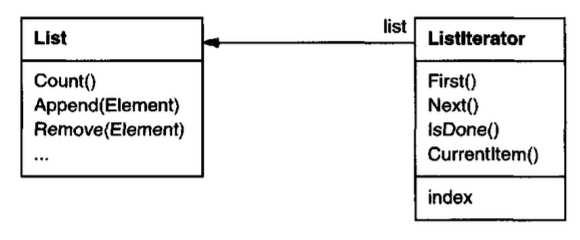
\includegraphics[width=0.5\linewidth]{assets/pattern/iterator/iterator-esempio-1.png}
\end{figure}

Il pattern Iterator ti permette di fare tutto questo prendendo la responsabilità dell'accesso e dell'attraversamento dall'oggetto lista e mettendola in un oggetto iteratore, dove la classe Iterator definisce un'interfaccia per accedere agli elementi della lista e un oggetto iteratore è responsabile di tenere traccia dell'elemento corrente, sapendo quali elementi sono già stati attraversati. Separare il meccanismo di attraversamento dall'oggetto List ci permette di definire iteratori per diverse politiche di attraversamento senza enumerarle nell'interfaccia List, ma notate che l'iteratore e la lista sono accoppiati e il cliente deve sapere che è una lista che viene attraversata invece di qualche altra struttura aggregata, quindi il cliente si impegna con una particolare struttura aggregata.

\begin{figure}[H]
    \centering
    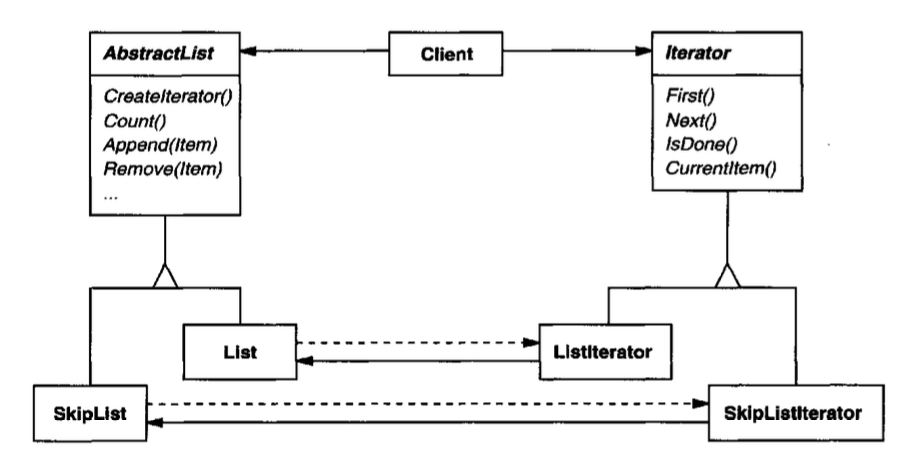
\includegraphics[width=0.75\linewidth]{assets/pattern/iterator/iterator-esempio-2.png}
\end{figure}

Sarebbe meglio se potessimo cambiare la classe aggregata senza cambiare il codice cliente, e possiamo farlo generalizzando il concetto di iteratore per supportare iterazione polimorfa definendo una classe AbstractList che fornisce un'interfaccia comune per manipolare liste e una classe Iterator astratta che definisce un'interfaccia di iterazione comune, permettendo poi di definire sottoclassi Iterator concrete per diverse implementazioni di lista, rendendo così il meccanismo di iterazione indipendente dalle classi aggregate concrete e usando un metodo factory come CreateIterator per connettere le due gerarchie di classi.

\paragraph{Applicabilità} È consigliabile utilizzare il pattern Iterator quando:
\begin{itemize}
    \item Si vuole accedere al contenuto di un oggetto aggregato senza esporne la rappresentazione interna;
    \item Si vogliono supportare più modi di attraversare oggetti aggregati.
    \item Si vuole fornire un'interfaccia uniforme per l'attraversamento di diverse strutture aggregate (ovvero, per supportare l'\textbf{iterazione polimorfica}).
\end{itemize}

\begin{figure}[H]
    \centering
    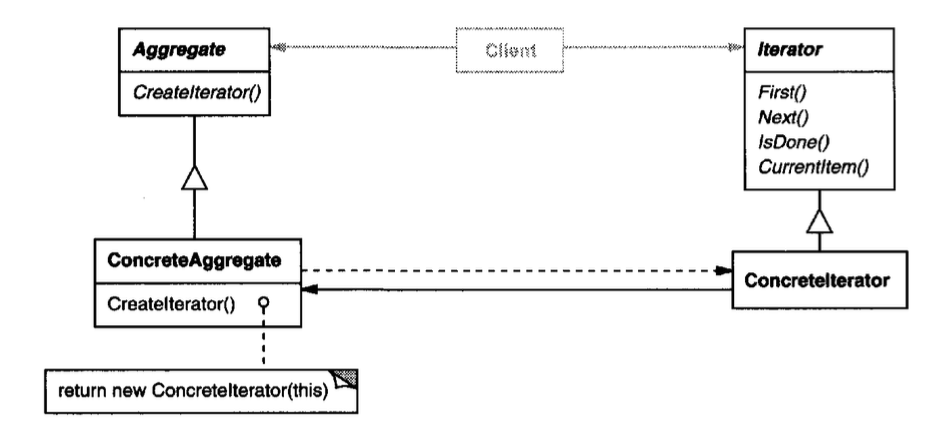
\includegraphics[width=0.75\linewidth]{assets/pattern/iterator/iterator-struttura.png}
    \caption{Class Diagram del pattern Iterator}
\end{figure}

\paragraph{Struttura} Il pattern Iterator è composto da:
\begin{itemize}
    \item \textbf{Iterator}: definisce un’interfaccia per attraversare l’insieme degli elementi di un contenitore e accedere ai singoli elementi.
    \item \textbf{ConcreteIterator}: implementa l’interfaccia Iterator tenendo traccia della posizione corrente nel contenitore e calcolando qual `e l’elemento successivo nella sequenza di attraversamento.
    \item \textbf{Aggregate}: definisce un’interfaccia per creare un oggetto Iterator.
    \item \textbf{ConcreteAggregate}: implementa l’interfaccia di creazione dell’Iterator e ritorna un’istanza appropriata di ConcreteIterator.
\end{itemize}

\paragraph{Conseguenze} Il pattern Iterator consente quindi di:
\begin{itemize}
    \item Semplificare l'interfaccia Aggregate: estraendo algoritmi di attraversamento voluminosi in classi separate.
    \item Supportare variazioni nell'attraversamento di un aggregato;
\end{itemize}

È bene notare che applicare il modello può risultare eccessivo se l'applicazione utilizza solo collezioni semplici (es. Liste, Set).

\begin{figure}[H]
    \centering
    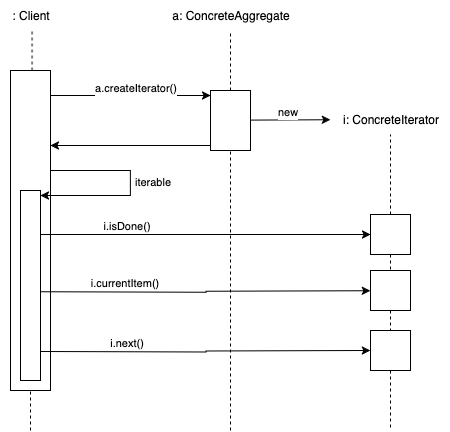
\includegraphics[width=0.75\linewidth]{assets/pattern/iterator/iterator-sequence.drawio.png}
    \caption{Sequence Diagram del pattern Iterator}
\end{figure}

ConcreteIterator posside un'istanza della collezione (passata a costruttore).

\newpage